
\subsection{Activity Configuration}
\label{sec:configuration}

Configuring an activity is the way to set parameters so that the activity occurs in the desired conditions.

In some cases developed in Section~\ref{sec:goals} (goals C and D in particular), configuration information is relevant to assess the quality and reliability of an activity or an entity, and to identify the location of configuration errors in a processing. It also facilitates the re-execution of an activity (reproducibility).

Configuration information may be carried by entities using the core features, where an entity (e.g. ValueEntity and DatasetEntity instances) is referenced in Used relations with a given role and type=“setup”. With this solution, the configuration information is independent from the activity and can be generated and used as any entity.

The data model also provides a specialized structure to directly attach configuration information to an activity. This structure is composed of a WasConfiguredBy relation with Parameter and ConfigFile objects (see~\ref{sec:configurationpackage}). With this solution the configuration information is independent from the entities, and seen as part of the activity.

%With the combination of those orientations, a project can select which pieces of configuration information is to be tracked, and which is to be simply attached to an activity.

%In some cases, it may be relevant to define all inputs as entities, following the pattern Activity-Used-Entity.

%In other cases, it may be relevant to attach configuration information directly and specifically to the activity, and define as entities only the objects that are to be traced.

%Access to configuration and access to provenance information are seen as different features of the model, the ActivityConfiguration part is thus kept separated from the execution and description parts of the model, even though they can have connections.

%Activity configuration typically implies a set of input parameters attached to the activity before execution, or a configuration file that contains those parameters. In order to link this detailed configuration with provenance information, a \class{Parameter} class is connected to the \class{Activity} class, along with a \class{ParameterDescription} class.


% Activity Configuration package overview
\begin{figure}[hbt]
\centering
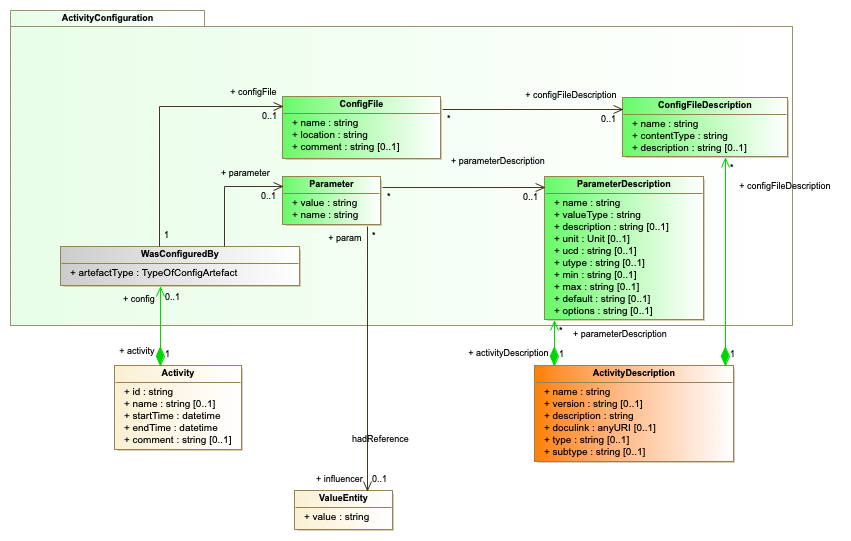
\includegraphics[width=1.0\textwidth]{figures/2019-05-28_ActivityConfiguration.png}
% Mireille: updated the diagram file for the last version with the proper cardinalities for Parameter and ConfigFile
\caption[Partial class diagram focused on the ActivityConfiguration package.]{Partial class diagram focused on the ActivityConfiguration package. The Parameter and ConfigFile classes provide configuration information for an Activity instance. The right side of the diagram shows the descriptions, where an ActivityDescription class is bound to its ParameterDescription and ConfigFileDescription classes.}
\label{fig:activityconfig}
\end{figure}
% classes attributes

\subsubsection{Overview of the ActivityConfiguration package} \label{sec:configurationpackage}

As shown in Figure \ref{fig:activityconfig} the \class{ActivityConfiguration} package contains two classes for the execution side: \class{Parameter} and \class{ConfigFile} which are connected to an \class{Activity} instance via the \class{WasConfiguredBy} association class.
An \class{Activity} may thus be configured by a set of \class{Parameter} instances, by a \class{ConfigFile} instance containing a list of (key,value) pairs, or by a combination of both.

% Mathieu: commented as it is about implementation
%The value stored in a \class{Parameter} can be explicitly queried while the values inside a \class{ConfigFile} need a search method for this.  This current standard does not provide the description for search methods and leaves it to the projects.

The corresponding description classes, \class{ParameterDescription} and  \class{ConfigFileDescription}, are both defined in the context of the description of an Activity.
There can be several instances of a \class{Parameter} (respectively \class{ConfigFile}) that are described by the same instance of  \class{ParameterDescription} (respectively \class{ConfigFileDescription}).
%, as the activities they configure may refer to the same ActivityDescription instance.

% Mathieu: commented as it is about implementation
%They are e.g. provided by the pipeline designer and filled in together with the \class{ActivityDescription}.
%This information can be imported from an external service which stores the documentation of the processing or observation methods applied in the activities of the project.

\subsubsection{Parameter and ParameterDescription classes}
\label{sec:parameterandD}

%The following attributes are defined to handle a Parameter instance and describe it.

\begin{table}[ht]
\small
\tymax  0.5\textwidth
 \textbf{\normalsize Parameter}\vspace{0.25em}\\
 \begin{tabulary}{1.0\textwidth}{llL}
 \toprule
 \head{Attribute} & \head{Data type}   & \head{Description}\\
 \midrule
%\textbf{id}   & string            & a unique id\\
\textbf{name} &  string & name of the parameter \\
\textbf{value} & string  & the value, type depends on \attribute{ParameterDescription.valueType} \\
\bottomrule
\end{tabulary}
\caption[Attributes of the \class{Parameter} class]{Attributes of the \class{Parameter} class. Attributes in \textbf{bold} must not be null.}
\label{tab:param}
\end{table}

\begin{table}[ht]
\small
\tymax  0.5\textwidth
\textbf{\normalsize ParameterDescription}\vspace{0.25em}\\
\begin{tabulary}{1.0\textwidth}{lLL}
 \toprule
 \head{Attribute} & \head{Data type}   & \head{Description}\\
 \midrule
%\textbf{id}  & string &  unique ParemeterDescription identifier\\
\textbf{name} & string & name of the parameter \\
\textbf{valueType} & string & VODML value type, see \citet{std:VODML} \\
description & string  & a descriptive text for the parameter \\
unit        & string  & physical unit, see \citet{std:VOUNIT} for recommended unit representation \\
ucd         & string  & Unified Content Descriptor, supplying a standardized classification of the physical quantity, see \citet{std:UCD13} \\
utype       & string  & Utype, meant to express the role of the parameter in the context of an external data model \\
% Mireille   removed the reference to the Utype note by Graham and al. not the definition of it but critics instead.
%xtype         & string & extended datatype as in VOTable 1.2 and above. A list of proposed \\
% \midrule
% \multicolumn{3}{@{}l}{\textbf{Optional attributes:}} \\
min         & string whose value can be interpreted by the valueType attribute & minimum value \\
max         & string whose value can be interpreted by the valueType attribute & maximum value\\
options     & string & comma separated list of possible values\\
default     & string whose value can be interpreted by the valueType attribute & the default value of the value entity \\
\bottomrule
\end{tabulary}
\caption[Attributes of the \class{ParameterDescription} class]{Attributes of the  \class{ParameterDescription} class. Attributes in \textbf{bold} must not be null.}
\label{tab:Paramdescription}
\end{table}

The \class{Parameter} class contains a \attribute{value} and a \attribute{name} attribute that must be set (Table~\ref{tab:param}).

The \class{ParameterDescription} class describes the parameter \attribute{value} attribute similarly to the \class{ValueEntity} and \class{ValueDescription} classes. Those attributes are listed in Table~\ref{tab:Paramdescription}.

If a \class{ParameterDescription} instance is defined, the \attribute{name} attribute of the related \class{Parameter} instances must match the \attribute{name} attribute of this \class{ParameterDescription} instance.


\subsubsection{ConfigFile and ConfigFileDescription classes}

\begin{table}[ht]
\small
\tymax  0.5\textwidth
 \textbf{\normalsize ConfigFile}\vspace{0.25em}\\
 \begin{tabulary}{1.0\textwidth}{llL}
 \toprule
 \head{Attribute} & \head{Data type}   & \head{Description}\\
 \midrule
%\textbf{id}   & string            & a unique id\\
\textbf{name} &  string & a human-readable name for the config file \\
\textbf{location} & string  &  a path to the config file, e.g. a URL \\
comment & string  & text containing comments on the config file  \\
\bottomrule
\end{tabulary}
\caption[Attributes of the \class{ConfigFile} class]{Attributes of the \class{ConfigFile} class. Attributes in \textbf{bold} must not be null.}
\label{tab:configfile}
\end{table}

\begin{table}[ht]
\small
\tymax  0.5\textwidth
\textbf{\normalsize ConfigFileDescription}\vspace{0.25em}\\
\begin{tabulary}{1.0\textwidth}{llL}
 \toprule
 \head{Attribute} & \head{Data type}   & \head{Description}\\
 \midrule
%\textbf{id}  & string &  unique ParemeterDescription identifier\\
\textbf{name}    & string & a human-readable name for the config file \\
\textbf{contentType}  & string  & MIME-type or format of the dataset \\
description     & string  & a descriptive text for the config file \\
\bottomrule
\end{tabulary}
\caption[Attributes of the \class{ConfigFileDescription} class]{Attributes of the  \class{ConfigFileDescription} class. Attributes in \textbf{bold} must not be null.}
\label{tab:configfiledescription}
\end{table}

The \class{ConfigFile} is a text file, where key value pairs are listed as parameters for running an Activity. It contains a \attribute{location} and a \attribute{name} that must be set, and a \attribute{comment} attribute (Table~\ref{tab:configfile}).

The \class{ConfigFileDescription} class indicates the format in which the list is provided in a \attribute{contentType} attribute (see Table~\ref{tab:configfiledescription}).

If a \class{ConfigFileDescription} instance is defined, the \attribute{name} attribute of the related \class{ConfigFile} instances must match the \attribute{name} attribute of this \class{ConfigFileDescription} instance.


\subsubsection{Relations with Activity Class}

The relation of \class{Parameter} and \class{ConfigFile} to \class{Activity} is formalized by a \class{WasConfiguredBy} class. This class contains the attribute \attribute{artefactType} that takes the value "Parameter" or "ConfigFile" (TypeOfConfigArtefact enumeration).

The life cycle of a \class{Parameter} instance (respectively \class{ConfigFile} instance) is the one of the corresponding \class{Activity} instance.
The life cycle of a \class{ParameterDescription} instance (respectively \class{ConfigFileDescription} instance) is the one of the corresponding \class{ActivityDescription} instance.
This means that when an activity is deleted from the provenance repository, its parameters and config files also disappear.

Several activities launched with various possible values for a parameter share the same \class{ParameterDescription} instance.
For instance, a cube analysis activity with a parameter "nbofChannels" will point to the corresponding instance of \class{ParameterDescription} (\attribute{name} = nbofChannels, \attribute{ucd} = meta.number, \attribute{unit} = NULL, \attribute{description} = ‘Nb of channel used for segmentation’).
% Mathieu: this part is about implementation
% Other implementation examples are provided together on the RFC page. See \url{https://wiki.ivoa.net/twiki/bin/view/IVOA/ProvFocusAstericsExamples}.

Similarly, we can foresee a number of different \class{ConfigFile} instances used for various instances of an \class{Activity}, which rely on the same \class{ConfigFileDescription} instance bound to the corresponding \class{ActivityDescription} instance.

%  ??? a deplacer vers la partie Description ??
% Mathieu: This suggest a dedicated serialisation of the description, explained in a separate document
%An \class{ActivityDescription} works as a template which binds to the configuration, to the top of the diagram and to the data flow represented in \class{UsageDescription} and \class{GenerationDescription} where the Entities consumed and produced by the ActivityDescription are designated with their role. Such a template can be imported from a project code repository, for instance.

%Some \class{Parameter} values may have been elaborated from a computation, a process which produced this value and can be part of the provenance information. In this case an \class{Activity} instance exists in the system that did produce a \class{ValueEntity} instance which contains this specific value.
The \class{Parameter} instance may refer to a \class{ValueEntity} instance using a \textit{hadReference} which gives the origin of this value.
